\documentclass{article}

\ifx\pdfoutput\undefined
% we are running LaTeX, not pdflatex
\usepackage{graphicx}
\else
% we are running pdflatex, so convert .eps files to .pdf
% pdflatex --shell-escape filename
\usepackage[pdftex]{graphicx}
\usepackage{epstopdf}
\fi

\usepackage{hyperref}
\usepackage{verbatim}
%\usepackage{amsmath}
%\usepackage{lscape}
\usepackage{wrapfig}

\begin{document}

\title{Cortana Manual}

\maketitle

%TODO
%binning vs all vs best - may need to go into separate section
%relation between attribute type and target type
%equations for target type seach condition tests
%double correlation
%multi-label
%search strategy
%result window
%search settings vs search parameters (form by conditions and strategy)
%NEW numerical operators, affect single numeric (or all Target Type settings)
%NEW nominal operator !=
%NEW HistogramWindow
%NEW CrossTableWindow
%NEW PlotWindow

%TODO move to actual Start section + ref CPJ
\section{Before you start}
\label{section:before}
Although Cortana is written in Java, and therefore platform independent, it will behave slightly different on different operation systems and/or platforms.
These differences arise from small variations in the Java Virtual Machines, used in different situations.
The main issue is with 32-bit operating systems (OS).
On such systems the maximum amount of memory the Java Virtual Machine (JVM) can use is around 1600 MegaBytes.
However, the actual amount depends on the amount of RAM available.
The cortana.bat and cortana.sh file included in the Cortana.zip set the maximum amount of memory the JVM can use to 1600 MegaBytes, through the -Xmx option.
The value should, at most, be set to half the amount of available RAM, meaning eg. for a 2GB machine to \emph{-Xmx1000m}.
For 64-bit OSes no such limit exists, and it should be save to remove the -Xmx.
Note that the above means that, especially for 32-bit OSes, not all datasets will fit into memory.
This is a problem particularly relevant to the bioinformatics setting (see section~\ref{usage:bioinformatics}), as some of the background sources used for enrichment are relatively large.
%TODO bioinformatics ref





\section{Preliminaries}
\label{section:preliminaries}
Before giving a detailed description of the functionalities of Cortana, it is beneficial to first clarify some of the terms used in the rest of this manual.



\subsection{Dataset}
\label{preliminaries:dataset}
First there is the data that will be used as input.
The data can often best be visualised as a table, or matrix, containing \emph{columns} and \emph{rows}.
The first \emph{row} of the data, the \emph{header}, contains all the names of the columns.
The remaining rows form the so-called instances, and describe, for each instance, the values for each \emph{column}.
Different authors use different names for the same concepts.
To be clear, a \emph{dataset} describes all data under investigation, and is referred to by some authors as \emph{population}.
The members that constitute a dataset are referred to as instances or \emph{examples}.
Columns will be referred to as \emph{attributes}, and the \emph{column name} is the \emph{attribute name}.

Currently, two types of files can be loaded into Cortana, ARFF files and plain (comma-separated) text files.
Both file types provide the data in a matrix form.
ARFF (\emph{Attribute-Relation File Format}) files, however, additionally define the data type, or \emph{attribute type}, of each attribute in a section preceding the actual data.
ARFF files are very common in data mining. More on them can be found at \url{http://www.cs.waikato.ac.nz/~ml/weka/arff.html}.



\subsection{Attribute Type}
\label{preliminaries:attribute-type}
Each attribute has an attribute type that indicates what kind of data is associated with the attribute.
Currently, Cortana distinguishes three attribute types: \emph{nominal}, \emph{numeric} and \emph{binary}.
This is less than the number of attribute types that can be declared in an ARFF file.
Some of the valid ARFF types are mapped to a valid Cortana attribute type.
For instance, the ARFF types \emph{numeric}, \emph{real} and \emph{integer} are all handled by Cortana as the \emph{numeric} attribute type.
An attribute with the \emph{nominal} attribute type is said to be a nominal attribute, and likewise for the other attribute types.
%String and date are not supported atm.



\subsection{Subgroup}
\label{preliminaries:subgroup}
A \emph{subgroup} is a selected number of instances from the dataset.
As returned by Cortana, it will both be non-empty, and will not contain all instances in the dataset.
Any \emph{Subgroup Discovery} process will try to find subgroups that, on a characteristic of interest, show a statistically unusual deviation from the whole dataset.



\subsection{Subgroup Discovery}
\label{preliminaties:subgroup-discovery}
Cortana is a generic Subgroup Discovery tool.
However, it differs from other such tools in some respects.
Traditionally, Subgroup Discovery could be described as a heuristic search process in which one tries to optimise for a single target attribute, or \emph{target value}, using some quality measure.
A \emph{target attribute}, or \emph{target} for short, should be understood as one of the attributes available in the dataset, and the target value, then, is one of the valid values for that attribute.

Note that for \emph{nominal} \emph{targets} the target value is contained in the data as one of its values.
For a \emph{numeric} \emph{target} however, one does not set a target value in Cortana, and the underlying Subgroup Discovery algorithm will, within the range determined for that \emph{target}, infer its own boundaries to create subgroups.
%reference boundary selection process



\subsection{Condition}
\label{preliminaries:condition}
A condition is a description, or the intension, of a subgroup, while the actual instances that form a subgroup constitute its extension.
The simplest, or atomic, condition consists of three parts: an attribute, an \emph{operator} and a value.
More complex conditions can be formed from conjunctions of atomic conditions.
\emph{Conjunctions} formed this way are sometimes also referred to as \emph{condition lists}.
An example of an atomic condition would be: $age \leq 18$, a more complex one would be $age \leq 18 \wedge length \leq 1.8$.



%TODO \Subsection{Operators} on Operators for different AttributeTypes



%TODO nr measures > 43
\subsection{Quality Measure}
\label{preliminatier:quality-measure}
In Subgroup Discovery, one uses a \emph{quality measure} to asses the quality of the subgroups found.
Here, \emph{quality} should be understood as a score obtained by appying the quality measure to, the characteristics of, the subgroup.
It depends on the actual quality measure, and/or the goal the researcher has in mind, whether such a \emph{quality} should evaluate high or low.
For example, if the very simple quality measure `\emph{average}' is used, it depends on the domain specific goal whether one would try to obtain a very high or low score.
Cortana features more than 40 quality measures, most based on statistical tests.
This manual currently does not provide a description of them, and the user is referred to any statistical handbook, or relevant papers from the data mining community, e.g. \cite{shb,remauv}.
%book



\subsection{Target Attribute vs. Target Concept}
\label{preliminaries:target-concept}
Traditionally, Subgroup Discovery focussed only on optimising for a single \emph{target}, or target value.
Obviously, this is a setting that can still be used in Cortana.
However, since Cortana can also be used in a novel setting referred to as \emph{Exceptional Model Mining} (\emph{EMM}) \cite{emm,sdmbn}, the object of optimisation need no longer be singular, and hence non-plural terms like \emph{target} and target value are no longer applicable.
Therefore the term \emph{target concept} is introduced.
In better describes what is the object of the optimisation effort used in the Subgroup Discovery process.
There are a number of target types related to target concepts.
Section \emph{Target Type}~\ref{preliminaries:target-type} describes them in more detail, including their influence on the Subgroup Discovery algorithm used by Cortana.



\subsection{Target Type}
\label{preliminaries:target-type}
%relation between attribute type and target type

\subsubsection{Single Nominal}
The first target type is \emph{single nominal}.
It may very well be the best known, and most used, target type in the Subgroup Discovery discipline.
In this setting, the target concept is simply one of the values of the target attribute, more commonly known as target value.
For most quality measures, Cortana will optimise the quality of subgroups by considering the proportion of positive and negative examples in the dataset.
\emph{Instances} count as positive examples if their value for the target attribute is identical to the target concept, they are negative otherwise.
Note that this yields a binary distinction, such that, for any target attribute, only that value that coincides with the target concept is considered positive, all other values, including \emph{missing values}, are considered negative.
%TODO So Cortana uses the following equality test to determine whether an instance is a positive example: \emph{instance.target-attribute.target-value equals target-concept}.
%TODO equals is =, or ==, also adres NEW != operator for NOMINAL

\subsubsection{Single Numeric}
The second target type is \emph{single numeric}.
This is another simple target type, however, it substantially differs from the \emph{single nominal} type.
Most importantly, one does set a single target attribute, but one does not set a target value when using this setting.

This target type can only be used for \emph{numeric} attributes.
All values of such attributes are numeric, and thus define a range.
The goal of the Subgroup Discovery process will then, most often, be to find a certain threshold value, within that range, that best separates the whole dataset into a subgroup and its complement, such that the distribution, on the target attribute, of that subgroup differs most from the distribution of the whole dataset.
Here the quality measure plays an important role, since it determines whether Cortana should try to find subgroups that have a much higher or lower average value for the target attribute than the average value for the whole dataset.
The simple quality measure `\emph{average}'  would try to miximise this value, while `\emph{inverse average}' would try to minimise it.

As alluded to above, in this target type setting, threshold values are inferred to form subgroups.
For a \emph{numeric attribute}, Cortana will test various threshold values to set apart instances, constituting a new subgroup, from the rest of the dataset.
Instead of an (in)equality test, as used in the \emph{single nominal} setting, Cortana uses can use, a combination of, different tests (`$<=$', `$>=$' and `$=$') to form subgroups in the \emph{single numeric} setting.
So, for a \emph{numeric attribute}, a threshold value is selected, and then, for each instance in the dataset, it is determined whether this instance is to be regarded as a positive or a negative example, based on the value of that instance and the actual test performed.
Eg., when using the `$<=$' test, an instance counts as a positive example if its value is less than, or equal to, the selected threshold, and negative otherwise.
Obviously, in case of the `$>=$' test an instance is regarded a positive example if its value is greater than, or equal to, the selected threshold, and considered a negative example otherwise.

The final point to address for this target type is to clarifying how Cortana actually determines the thresholds it uses.
Unfortunately, there is no short answer to this question, as it depends on the actual \emph{search strategy} selected by the end user.
However, for all three \emph{best numeric} \emph{search strategy} types, Cortana selects as threshold a value from the data range of the \emph{numeric attribute} under consideration.
For more details on \emph{search strategy}, see section~\ref{main:search-strategy}.
%binning vs all vs best - may need to go into separate section

\subsubsection{Double Correlation}
This target type is used in one of \emph{Cortana's} implementations of possible \emph{Exceptional Model Mining} extentions of traditional Subgroup Discovery.
More on \emph{Exceptional Model Mining} in general, and some of its possible implementations, can be found in Leman, Feelders, Knobbe (2008)~\cite{emm}, and the ideas presented there will not be reiterated in this manual.
However, as the purpose of this manual is to provide some useful, or necessary, information about, parts of,  Cortana, a little will be said about this target type, its use, and the way it influences the Subgroup Discovery process used by Cortana to form candidate subgroups.
%TODO

\subsubsection{Multi-label}
%TODO


\section{Starting Cortana}
After obtaining and unpacking a copy of Cortana from \url{http://datamining.liacs.nl/cortana.html}, navigate to the Cortana directory.
There you will find a cortana.jar file.
One could start Cortana by double clicking the jar, however, it is recommended to start Cortana from the command line.
This way, a lot more information about the Subgroup Discovery process is fed back to the user.
To start Cortana this way, open a terminal or command window, navigate to the Cortana directory containing cortana.jar, and type: \emph{java -jar cortana.jar}.
Alternatively one can use either cortana.bat (for Windows) or cortana.sh (Bash shell script).
Be sure to read Section~\ref{section:before} \emph{Before you start} if you do.

After starting Cortana one is asked to select the file that contains the dataset to be analysed, after which Cortana's main screen is shown.

%TODO implement quickie separator guess code
Currently, two types of files can be loaded into Cortana, ARFF files and plain (comma seperated) text files.
The first is very common in data mining and describes the data and additionally defines the attribute type of each attribute.
As such, ARFF files are preferred over plain text files.
For text files, Cortana wil try to infer the correct attribute type of each attribute.
Unfortunately, this may fail, so to check whether Cortana was able to infer the correct attribute type, or change the attribute type anyway, the \emph{Meta Data...} button on the main screen gives access to the \emph{Meta Data Window} (section~\ref{section:meta-data-window}).





\section{Cortana - Main Screen}
\label{section:main}
The main screen of Cortana is devided into four major panels, \emph{Dataset}, \emph{Target Concept}, \emph{Search Conditions}, and \emph{Search Strategy}.
The following subsections will address them all.

\begin{figure}
\begin{center}
\centering
\resizebox{1\columnwidth}{!}{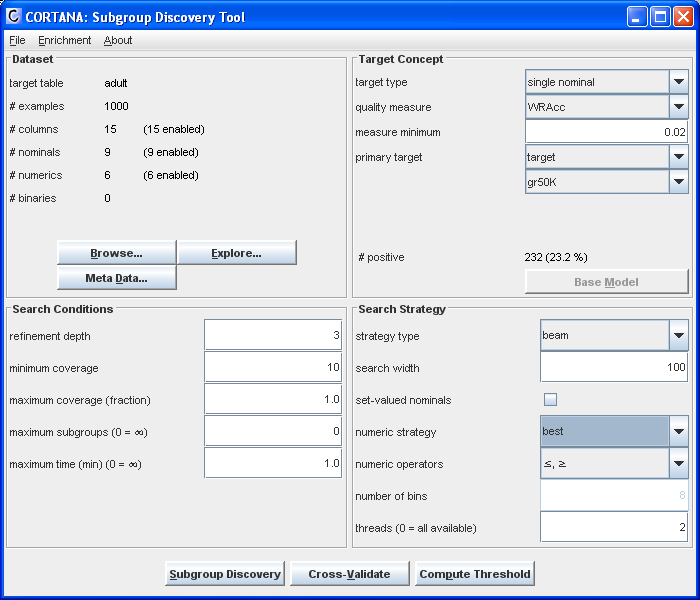
\includegraphics{mainwindow.png}}
\caption{Cortana's main window.}
\end{center}
\label{fig:mainwindow}
\end{figure}


\subsection{Dataset}
\label{main:dataset}
As can be expected from the name, this panel gives some information about the dataset that is currently loaded.

{\bf target table} shows the name of the data file used, which for text files is just the filename, and for ARFF files is the name defined in the '@relation' field.

{\bf\# examples} shows the number of examples in the dataset.

{\bf\# columns} shows the number of columns in the dataset.
Remember that columns are also be referred to as attributes.

Finally, there is a number of fields that indicate the number of attributes from each data type.
The type of an attribute determines the sort of mining algorithm or quality measure that is applicable to it.
More about this can be found in section~\ref{preliminaries:attribute-type}.

In addition to the fields described above, there are three buttons present on the {\bf Dataset} panel, {\bf Browse...}, {\bf Meta Data...} and {\bf Explore...}.

By clicking the {\bf Browse...} button, a Browse Window (section~\ref{section:browse-window}) is presented, showing a table with the data in the state that it is currently in.
Additionally, in the table header, it shows the number of distinct values for each attribute.
Note that the data may not be in the same state as when it was loaded, as it can be modified using functionality of the Meta Data Window, presented after pressing the {\bf Meta Data...} button, which is also present on the {\bf Dataset} panel.
Section~\ref{section:meta-data-window} describes the Meta Data Window, its components, and the data manipulation functionalities, in more detail.

{\bf Explore...} button.

\begin{figure}
\begin{center}
\centering
\resizebox{0.5\columnwidth}{!}{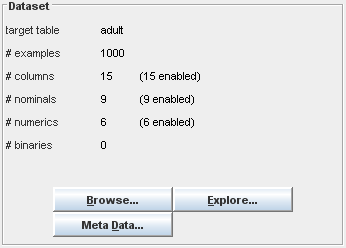
\includegraphics{dataset.png}}
\caption{Dataset details in the main window.}
\end{center}
\label{fig:dataset}
\end{figure}





\subsection{Target Concept}
\label{main:target-concept}
%TODO clean up, contains double info
The fields of this panel serve to manipulate the target concept-related search settings used during the Subgroup Discovery process.
Traditionally, Subgroup Discovery focused only on optimising for a single target attribute.
Obviously, this is a setting that can still be used in Cortana.
However, since Cortana can also be used in a novel setting referred to as \emph{Exceptional Model Mining} (\emph{EMM}) \cite{emm}, the term target value is no longer applicable, hence the term \emph{Target Concept}.
Section~\ref{preliminaries:target-type} describes the various target types in more detail.
In this section only a short description of the various fields will be given.

The first field is {\bf target type}, that is used to change the target type for which one wants to do Subgroup Discovery.
Selecting another target type from the drop down box will force Cortana to consider other attributes as target concept.
For example, when changing the target type from the default \emph{single nominal} to \emph{single numeric}, the first attribute having the numeric attribute type is selected, and subsequently displayed in the {\bf primary target} drop down box.

Based on the target type selected, a number of quality measures is available.
These are listed in the {\bf quality measure} drop down box.
After changing the target type, the quality measures listed in the {\bf quality measure} drop down box are automatically updated, to fit the new target type.

The text field next to {\bf measure minimum} will, show a minimum threshold value for the selected quality measure.
One might consider lowering this value if a Subgroup Discovery experiment, run with the default value, returned too few subgroups.
On the other hand, one can increase this value to force Cortana to only report subgroups that have a sufficiently quality.

\begin{figure}
\begin{center}
\centering
\resizebox{0.5\columnwidth}{!}{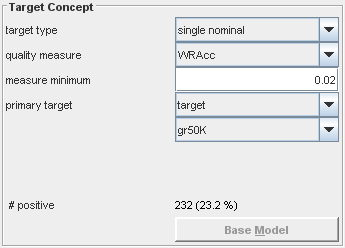
\includegraphics{targetconcept.png}}
\caption{The target concept specification details in the main window.}
\end{center}
\label{fig:targetconcept}
\end{figure}


\begin{comment}
It might be better to present the following fields on a per terget type basis, mentioning, for each target type, only the relavant fields, and their characteristics in relation to that target type.
In code, do not show double correlation if #numerics < 2.
Also, for secondary target select 2nd numeric attribute by default, not first.
In code, do not show multi-label if #binaries < 2.
In code, do not show irrelevant target types based on data set characteristics.
In code, maximum time <= 0, means unlimited time, like in ...
\end{comment}



The items described in the remainder of this section will not be available in every target type setting, as the various target types are related to the attribute type of the target concept.
For each item, it will be mentioned to which attribute type it applies.

\textbf{primary target} is available in the following target type settings: \emph{single nominal}, \emph{single numeric} and \emph{double correlation}.
The {\bf primary target} drop down box lists all attributes available in the dataset.

\textbf{target value} is available only in the \emph{single nominal} setting.
The {\bf target value} drop down box lists all values of the attribute set as \emph{primary target}, which can be of the \emph{nominal} and \emph{binary} attribute type.

\textbf{secondary target} is available only in the \emph{double correlation} setting.
In this setting only attributes of the \emph{numeric} attribute type will be listed in both the \textbf{primary target} and {\bf secondary target} drop down box.

%TODO \section{Targets and Settings}
The \textbf{targets and settings} button is available only in the \emph{multi-label} setting.
If this target type is selected, the {\bf Targets and Settings} button will be enabled, and this gives access to the \emph{Multi-label details}.
The upper part of which shows some input fields related to multi-label search settings.
The lower part lists all attributes of the \emph{binary} attribute type.
More on the \emph{multi-label} can be found in section~\ref{section:multi-label} and in \cite{emm,sdmbn}.

Then, there is an information field that shows information relevant to the selected target type.
The number of positives, \textbf{\# positives} is shown for the \emph{single nominal} target type, \textbf{average} for \emph{single numeric}, \textbf{correlation} for \emph{double correlation} and \textbf{\# binary targets} for \emph{multi-label}.

%TODO \Section{Base Model}
The \textbf{Base Model} button will only be enabled if the target type is \emph{double correlation} or \emph{multi-label}.
It gives access to a \emph{Base Model Window}, showing a correlation plot for the selected primary and secondary target, if the target type is \emph{double correlation}.
For the \emph{multi-label} target type, it will show a \emph{bayesian network}, connecting the various binary attributes.







\subsection{Search Conditions}
\label{main:search-conditions}

The fields on this panel allow setting the search conditions used in the Subgroup Discovery process.
For all fields the default values are also given.

\textbf{refinement depth} controls the number of conditions that is used to create subgroups.
A refinement depth of $1$ would lead to conditions like $x \leq 9.11$, while a refinement depth of $2$ would allow for the creation of conditions like $x \leq 1.2 \wedge y \geq 3.4$.
It is not recommended to set the refinement depth to very high values.
In Subgroup Discovery, often a depth greater than $4$ or $5$ does not lead to significant improvements of the measure score any more, and just increases both the risk if overfitting, and the computational time needed to calculate the result.

\textbf{minimum coverage} sets the lower bound for the size of the subgroups that should be reported by Cortana, meaning all reported subgroups have at least this size.
The default value is set to $10\%$ of the total dataset size, which is shown as \textbf{\# examples}, see section~\ref{main:dataset} above.

\textbf{coverage fraction} sets the upper bound for the size of the subgroups that should be reported by Cortana, meaning all reported subgroups have at most this size.
The default value is set to $1.0$, which indicates the entire dataset.

\textbf{maximum subgroups} is used to control the maximum number of subgroups in the result list generated by Cortana.
First, this means that the Result Window (section~\ref{section:result-window}) will show at most this number of subgroups.
%Search width.

But also, as alluded to in the \emph{Dataset} section (\ref{main:dataset} on \emph{measure minimum}, this number also controls the number of intermediate results retained by Cortana to form the pool out of which the generation for the next \emph{refinement depth} is formed.
As such, this \emph{Search Condition} parameter has significant influence on the computational demands, as it directly controls the number of combinatorial candidates to be tested during Cortana's Subgroup Discovery process.
Without going into the actual algorithm, a small example probably suffices to make this clear.
For a dataset consisting of only \emph{nominal} attributes, assume $n =$ \emph{maximum subgroups}, and $m =$ \emph{number of attribute-value pairs}, then the number of candidates $c$ to be tested by Cortana for the next \emph{refinement depth} iteration is: $c = n \cdot m$.
%TODO calculation is incorrect, especially with new operator settings.
%Mention search strategies.

\textbf{maximum time (min)} will determine the maximum time, measured in minutes, Cortana is allowed to search for new subgroups.
After this periode Cortana will abort the Subgroup Discovery process and report all subgroups found up until that point.
This means that especially for the \emph{search strategy} (section~\ref{main:search-strategy}) \emph{strategy type} \emph{depth first} a large of the search space will not be explored at all, if the search proces is aborted.
More precisely, only the first attributes will have been addressed at that time.

\begin{figure}
\begin{center}
\centering
\resizebox{0.5\columnwidth}{!}{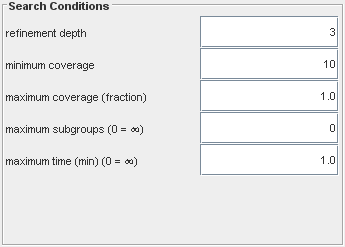
\includegraphics{searchconditions.png}}
\caption{Specification of the search conditions in the main window.}
\end{center}
\label{fig:searchconditions}
\end{figure}



\subsection{Search Strategy}
\label{main:search-strategy}
%TODO
This is an intro.
It describes \emph{strategy type}, \emph{best numeric} and \emph{number of bins}.

\textbf{strategy type} \emph{beam}, \emph{cover-based beam selection}, \emph{best first}, \emph{depth first} and \emph{breadth first}.
The default value is \emph{beam}.

\textbf{search width} This parameter can not be set for the \emph{best first} \emph{strategy type}.
The default value is \emph{$100$}.

\textbf{numeric operators} The default value is \mbox{\textbf{$<=$, $>=$}}.

\textbf{best numeric} \emph{bins}, \emph{best} and \emph{all}.
The default value is \emph{bins}.

\textbf{number of bins} Only available for the \emph{best numeric} setting of \emph{bins}.
Default value is \emph{$8$}.

\begin{figure}
\begin{center}
\centering
\resizebox{0.5\columnwidth}{!}{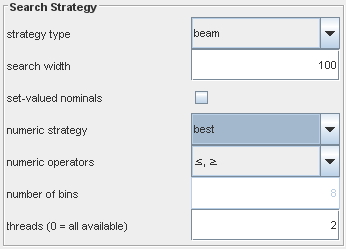
\includegraphics{searchstrategy.png}}
\caption{Search strategy specification in the main window.}
\end{center}
\label{fig:searchstrategy}
\end{figure}






\section{Browse Window}
\label{section:browse-window}
%use of save button in bioinformatics setting (may be made available in every setting to allow saving altered data)
%true positives button in single nominal setting for browse subgroup window
%search

\begin{figure}
\begin{center}
\centering
\resizebox{1\columnwidth}{!}{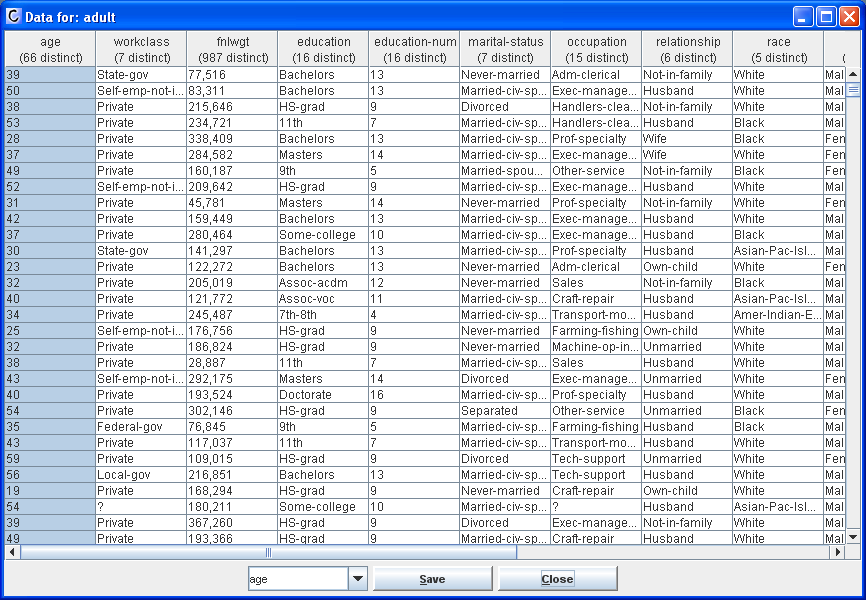
\includegraphics{browsewindow.png}}
\caption{The browse window.}
\end{center}
\label{fig:browsewindow}
\end{figure}




\section{Meta Data Window}
\label{section:meta-data-window}
The \textbf{Meta Data...} button gives access to a new window that, next to displaying some additional information about the dataset loaded, also allows changing some of the (characteristics of) the data.
The upper part of the \emph{Meta Data Window} shows a table with six columns.
The lower part contains a number of panels that allow modification of the data as it is in memory, note that no modifications are made to the original data file.
First the properties shown in the table in the upper part will be described, the purpose of the various data manipulations will be explained after that.

\begin{figure}
\begin{center}
\centering
\resizebox{1\columnwidth}{!}{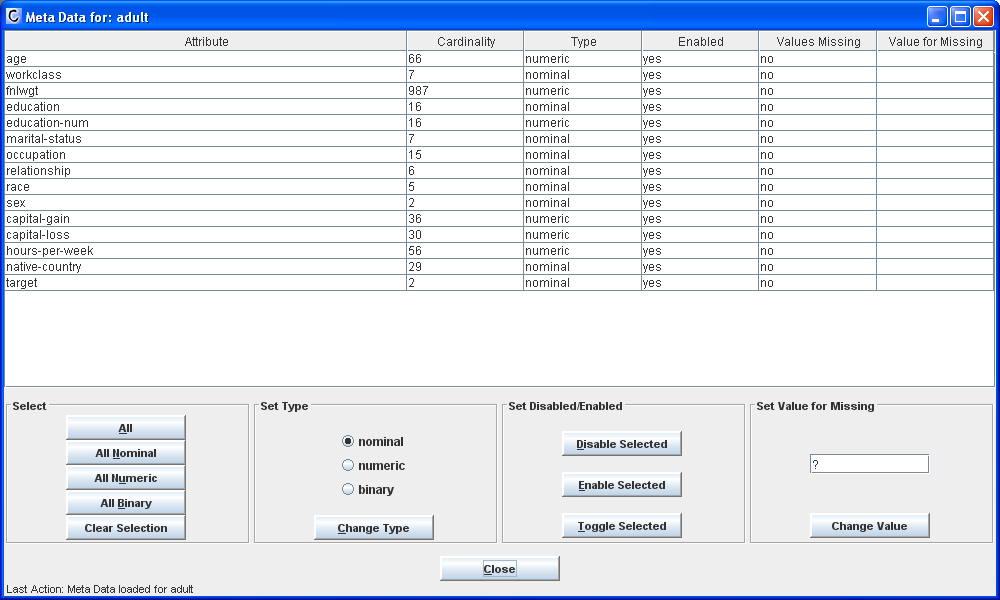
\includegraphics{metadatawindow.png}}
\caption{Meta data window.}
\end{center}
\label{fig:metadatawindow}
\end{figure}



\subsection{Meta Data Table}
\label{meta-data-window:meta-data-table}
The first column in this table, \emph{Attribute}, lists all \emph{attribute names} of the attributes in the dataset.
The remaining columns show some information for each of these attributes.
\emph{Cardiality} gives the number of distinct values for an attribute.
\emph{Type} shows its attribute type.
\emph{Enabled} indicates whether the attribute is \emph{enabled} or \emph{disabled}.
\emph{Values Missing} indicates whether the attribute contains missing values or not.
And finally, \emph{Missing Value} shows the value that is currently used for missing values in the data.
Obviously, this field is blank if there are no values missing for the attribute.

\subsection{Meta Data Functions}
\label{meta-data-window:meta-data-functions}
The panels in the lower part of the \emph{Meta Data Window} all allow selecting or changing the data.
The first, \emph{Select}, allows selecting all attributes of a certain type.
This is a conveiniance method to be used in combination with the functionalities available in other panels.

\textbf{Set Type} allows changing the attribute type.
This can be useful for various reasons.
The first is that, after loading a plain text file, it is observed that Cortana was not capable to infer the correct type for an attribute.
Related to this is the possiblity to change the type of an attribute to allow other quality measures to be used in the Subgroup Discovery process.
An example of this would be an attribute that describes the number of doors in a car dataset.
If this value is used as a target value, one might treat it as a \emph{nominal} property, forcing the Subgroup Discovery process to only perform equality tests on this \emph{attribute value} for the creation of the conditions used to form subgroups.
\emph{Instances} in the dataset are then either in the target set if they have the same value for the `doors' attribute as the selected target value, or are in the complement of the set formed by those instances.
If the `doors' attribute is treated as \emph{numeric}, any, combination, of the `$<=$', `$>=$' and `$=$' tests can used to create conditions to perform on the \emph{attribute values}.
This means that the size of the set of instances selected using an \emph{attribute value} might be bigger than in the \emph{nominal} case.
A condition using $doors >= 2$ will select all cars having two or more doors.
In the \emph{nominal} case it would not be possible to select this group using only one condition (assuming the set of cars having more than two doors is not empty).
Obviously, it would be possible to select the same group using a set of conditions like $doors equals `2' \vee doors equals `3' \ldots$, but, among other negative characteristics, creating such conditions would be computationally more demanding, and less intuitive.
Note that if there are missing values for an attribute, the \emph{missing value} value for this attribute might be automaticaly changed to a value that is relevant to the attribute type.
See \emph{Set Value for Missing} below for more on the \emph{missing value} values for the different attribute types.
%\ref{subsubsection:set-missing-values}

\textbf{Set Disabled/Enabled} allows to disable or enable an attribute.
When an attribute is disabled, it will not be considered by the mining algorithm to form conditions with to create subgroups.
Note that disabling an attribute does not affect the possiblity to select it as a target concept (see section~\ref{preliminaries:target-concept} for more on target concepts).

\textbf{Set Value for Missing} can be used to change the value that is curently used for values that were missing in the data.
The value that is used for missing values depends on the type of the attribute.
If, in an ARFF file, values are declared missing, using the `\emph{?}' directive, Cortana's file loader might replace this value with one that makes more sense in its Subgroup Discovery setting.
For \emph{nominal} types it will leave this value as is.
This will result in `\emph{?}' being one of the possible target values one can select for the corresponding attribute.
However, one can assign a diffent value to the \emph{missing values}.
One than has two options, either assign the \emph{missing values} a value that is an existing one for the attribute, or a non-exiting one.
In the first case one effectively assigns all instances that have a missing value for the corresponding attribute to one of the other \emph{attribute values}.
In the latter case, one just changes the value.
When changing the \emph{missing value} value of an attribute, the \emph{Cardinality} column is updated accordingly.
For \emph{numeric} and \emph{binary} attribute types Cortana's file loader will replace `\emph{?}' values with $0.0$ and $false$, respectively.
Again, if this is incorrect, or one wishes to assign the \emph{missing values} another \emph{attribute value}, either existing or non-existing, this can be done analogously to the \emph{nominal} case.
%Mention automatic missing value update on attribute type change.
%TODO valid values for each AttributeTypes





%TODO
\section{Multi-label}
\label{section:multi-label}





\section{Result Window}
\label{section:result-window}
When a mining run terminates, a \emph{Result Window} is shown.
The titlebar of this window shows some basic information about the search settings that were used to obtain the result displayed.
The top half of a \emph{Result Window} shows a table with the subgroups found, the lower half contains two rows of buttons.
Some of these buttons will be presented only in certain search settings.
Also, a number of buttons is used for post-processing, others just give access to additional information.
Finally, the buttons in the lower row will execute operations on the whole result set, that is all results shown in the Result Window, while those in the upper row operate only on the selected subgroup(s).

The following subsections will go into detail about the use of the various components of the Result Window.

\begin{figure}
\begin{center}
\centering
\resizebox{1\columnwidth}{!}{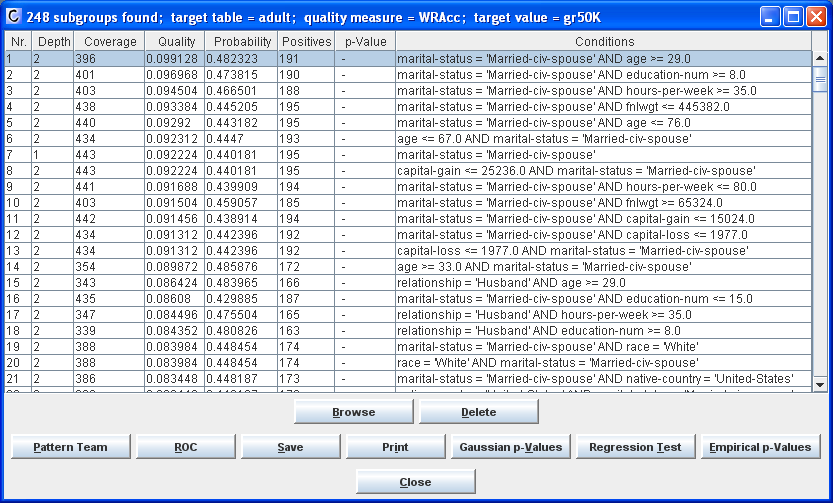
\includegraphics{resultwindow.png}}
\caption{The result window.}
\end{center}
\label{fig:resultwindow}
\end{figure}


\subsection{Result Set Table}
\label{result-window:result-set-table}
The top half of the Result Window consists of a Result Set Table, showing all subgroups in the result set.
From left to right the columns in this table are: \textbf{Nr.}, \textbf{Depth}, \textbf{Coverage}, \textbf{Measure}, \textbf{p-Value} and \textbf{Conditions}, and they all reveil a characteristic of the subgroup found.
This section will address all columns, and explains how to interpret the information they display.

\textbf{Nr.} shows the rank of the subgroup.
Note, however, that Cortana does not use a partial ranking for ties, and, as a result, subgroups that attain the same measure score, will not receive equal ranks.
Rather, if such an event occurs, Cortana assigns the value, displayed by \textbf{Nr.}, based on where in the Subgroup Discovery process the subgroup was found.

\textbf{Depth} shows the \emph{refinement depth} at which the subgroup was found.
As explained in the section on \emph{Search Conditions} (\ref{main:search-conditions}), the refinement depth controls the number of conditions that is used to create a subgroup.
So, a subgroup that is formed by using only one condition is said to have been found at depth $1$.
The number displayed at \textbf{Depth} is the same as the number of conjuncts in the \textbf{Conditions} column of the Result Set Table.

Note that in Subgroup Discovery it often happens that one condition already selects a highly valuable, high scoring, subgroup.
Adding extra conditions to this first one may improve the measure score, but only by a, possibly very, limited amount.
This will lead to a \emph{result set} containing a number of subgroups that all consist of the same 'base' condition, which is then refined with additional conditions using another attribute.
If these extra conditions do not substantially increase the measure score, all of these variations will attain consecutive ranks in the final result set.

\textbf{Coverage} shows the number of instances in the subgroup.
Depending on the target type used, this number can consist of both \emph{true positives} and \emph{false positives}, or just indicates the total size of the subgroup.

\textbf{Measure} shows the score of the subgroup, according to the quality measure used.
Different quality measures have different ranges for the scores they asssign to the worst and best possible subgroups.
As a result, measure scores resulting from applying different quality measures can not be compared directly in any sensible manner.
%ref wouter comparison paper

\textbf{p-Value} is initially blank.
But it will show the p-value of the subgroup after additional user input.
In Subgroup Discovery, quality measures are used that are based on, or insired by, well known, standard, statistical tests.
However, Cortana does not allow calculation of p-values in a fashion that is customary in statistics.
To be able to do so, the dataset under investigation should be considered a sample of the total population itself.
But, as the dataset is not treated as such, the calculation of the p-value is done using a different paradigm.
The major benefit of this paradigm is that it is agnostic to the target type used in the Subgroup Discovery process.
Section~\ref{result-window:p} \emph{Compute p-Value} below describes how the p-value is calculated in Cortana.
% ref thesis barbara p-value
% ref wouter p-value

\textbf{Conditions} shows the condition(s) used to form a subgroup.
As explained in Section~\ref{preliminaries:condition}, a condition consists of an attribute, an operator, and a value.
For depths greater than $1$, \textbf{Conditions} shows a conjunction of such conditions.



\subsection{Subgroup Buttons}
\label{result-window:subgroup-buttons}
The following subsections describe the various buttons that can appear on the upper row of the lower part of the \emph{Result Window}.
These buttons operate only on the subgroup(s) that are selected, or highlighted, in the \emph{Result Set Table}.
The selection can be changed using the mouse or pressing (Shift) and the Down/Up arrow of the keyboard.
The target type setting used for the Subgroup Discovery experiment determines which buttons will be shown.
For all buttons it will be indicated for what target type setting it is applicable.



\subsubsection{Show Model}
\label{result-window:model}
\textbf{Show Model} is available only for the \emph{multi-label} target type.
For all subgroups selected in the \emph{Result Set Table}, it will show a new \emph{Model Window}, depicting the bayesian network connecting the \emph{binary} attributes, according to the model that was inferred through the Subgroup Discovery process.



\subsubsection{Browse Subgroup}
\label{result-window:browse}
\textbf{Browse Subgroup} is available for all target types and will show a Browse Window as described in the Browse Window section (\ref{section:browse-window}).
For all subgroups selected in the Result Set Table, it will show such a window, depicting all instances that constitute the subgroup.
For the \emph{single nominal} target type one additional button is available, the \textbf{True Positives} button.
Clicking it will highlight only those instances that count as true positives.



\subsubsection{Delete Subgroup}
\label{result-window:delete}
\textbf{Delete Subgroup} is available for all target types and deletes a subgroup from the result set.



\subsection{Result Set Buttons}
\label{result-window:result-set-buttons}
The following subsections describe the various buttons that can appear on the lower row of the lower part of the Result Window.
These buttons operate on the whole result set, that is, on all subgroups in the result set.
As such, the results of these operations are unaffected by, changes in, the selection of subgroups in the Result Set Table.
The target type setting used for the Subgroup Discovery experiment determines which buttons will be shown.
For all buttons it will be indicated for what target type setting it is applicable.


\subsubsection{ROC}
\label{result-window:roc}
\textbf{ROC} is only available for the \emph{single nominal} target type.
All subgroups in the Result Set Table will be taken into account to show a \emph{ROC Curve Window}.
ROC (Receiver Operating Characteristic) curves have their origin in electrival engeneering, where they are used to show the performance of classifiers.
In the \emph{single nominal} setting some of the members of a subgroup are \emph{true positives}, while others are \emph{false positives}.
In a ROC plot the \emph{true positive rate} (TPR) of each subgroup is plotted against its \emph{false positive rate} (FPR).
When this is done, a line, the ROC curve, can be draw that forms a convex hull connecting the outer most points.
A straight diagonal from the lower left corner to the upper right indicates complete randomness of the result, and the furher the line approaches the upper left corner the better the result.
For a subgroup to reach the upper left corner, its TPR must be $1$, and its FPR $0$.

\begin{figure}
\begin{center}
\centering
\resizebox{1\columnwidth}{!}{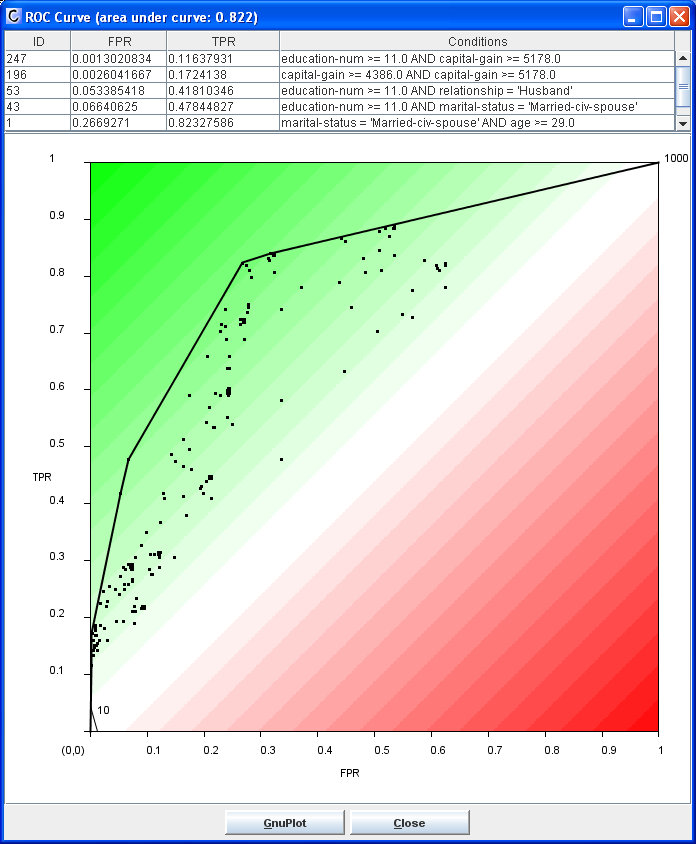
\includegraphics{rocwindow.png}}
\caption{The ROC window.}
\end{center}
\label{fig:rocwindow}
\end{figure}



\subsubsection{Compute p-Values}
\label{result-window:p}
To calculate the p-values for the subgroups found, the end user clicks the \textbf{Compute p-Value} button on the \textbf{Button Panel}.
In short the calculation of p-values is done by creating n random subgroups ...
%TODO explain

\begin{figure}
\begin{center}
\centering
\resizebox{0.3\columnwidth}{!}{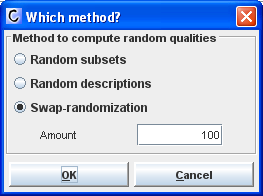
\includegraphics{randomizationdialog.png}}
\caption{Choosing the type of randomization to be used for any significance testing.}
\end{center}
\label{fig:randomizationdialog}
\end{figure}



\subsubsection{Regression Test}
\label{result-window:regression}
TBI.



\subsubsection{Empirical p-Values}
\label{result-window:empirical-p}
This functionality may be removed.



\subsubsection{Fold}
\label{result-window:fold}
TBI.



\subsection{Save}
\label{result-window:save}
\textbf{Save} is available for all target types.
It allows saving of the whole result set to a file.
The user will be asked for a name and location of this file.
The file will contain the information as it is depicted in the Result Set Table, and the values for the various columns will be comma-separated.



\subsubsection{Print}
\label{result-window:print}
\textbf{Print} is available for all target types.
It allows printing of the whole Result Set Table.
Note that it does not have a maximum amount of result it prints, the Result Set Table will be printed as-is.
Therefore, it is not recommended to use this functionality on large Result Sets.



\subsubsection{Close}
\label{result-window:close}
\textbf{Close} is available for all target types, and it will close the \emph{Result Window}.
Note that it can not be reopened.
Therefore, all necessary actions like, saving or printing the results, should be done before closing the Result Window.
All results will be lost, and the only way to get a new Result Window is to run the same Subgroup Discovery process again.
As this may be a very lengthy process, be sure to finish all operations before closing the Result Window.





\section{Usage}
\label{section:usage}



\subsection{Orinary Subgroup Discovery}
\label{usage:normal}
java -jar Cortana.jar



\subsection{Bioinformatics Setting}
\label{usage:bioinformatics}





\section{Autorun}
\label{section:auto-run}
Cortana comes with the ability to run experiments in an unsupervised setting.
This is a mode that is specifically created to allow so-called batch mining.
This section will explain how Cortana accomplishes this, and how to set up an \emph{autorun} or batch mining experiment.

In normal usage mode, the end user can set all search settings using the graphical user interface (GUI).
After loading a data file and setting the search settings one usually clicks the Subgroup Discovery button, and the Subgroup Discovery process begins.
However, Cortana's menu bar on the top of the main window gives access to two options that allow saving the search parameters to a XML-file.
This file can then be used to start the Subgroup Discovery process, using the defined search settings, at some other time.

The two autorun related options can be found under the \textbf{File} menu, and are named \textbf{Create Autorun File} and \textbf{Add to Autorun File}.
The first will ask the user for a name and location for the new file that will be created, containing all information, as shown in the main window, needed to do an unsupervised Subgroup Discovery experiment.
The second option allows to add all information currently presented by the main window to an already existing autorun file.
By using this last option one can create a large file, containing multiple experiments.
An example usage would be running several experiments on a single data file, where each experiment uses a different quality measure.

The paragraph above refers to information, and not solely search settings, as the XML-file used in the \emph{autorun} setting also needs to know the name of the data file to use.
That name is not part of the search settings, but it is important to state how Cortana looks for this data file.
When loading the autorun XML-file, Cortana will remember the directory in which this autorun file resides.
It will then parse the XML-file, and retrieve the name of the data file to use.
Cortana will then try to load the data file from the directory in which the autorun resides, and that directory only.
This means no relative paths can be used for the location of the data file, and the autorun file should always reside in the same directory as the data file(s) for which it describes experiments.
Although this limits its use, it keeps it easily portable, as, in this way, one can simply exchange directories containing autorun file(s) and accompanying data file(s), without having to worry about setting paths correctly in the autorun file, or placing the directories in the correct relative location, before being able to run an experiment.

When Cortana runs an experiment defined in an autorun file, the Subgroup Discovery process is exactly the same as when the experiment would be started from the GUI.
However, at the end of the Subgroup Discovery process, there are a few deviations from the normal GUI situation.

First of all, when the Subgroup Discovery process terminates, the Result Set will be automatically saved, as it would happen when the end used clicks the \textbf{Save} button in the Result Window.
The result file will have a name indicative of the search settings used, and starts with the data file name.
Also, it will contain a time stamp as part of its name, so that identical runs on, updated versions of, the data file will not overwrite older results.
The result file will be saved to the directory in which the autorun file resides.

Second, a Result Window may or may not be shown.
Whether it is, is controlled by a command line parameter, as shown at the end of this section.
Omitting this command line parameter will cause Cortana to default to always showing a Result Window after an experiment finishes.
Showing the \emph{Result Window} is necessary if one wishes to perform additional actions on the result set, be it plotting ROC Curve Windows, calculating p-Values or any of the other actions described in Section~\ref{section:result-window}.

Third, if the autorun file defined multiple experiments, the next experiment will be run automatically.
This will go on until all the experiments in the autorun file are executed.
In case of any errors, for example when Cortana can not locate a data file, some efforts are made to resume execution by discarding the erroneous experiment and continuing with the next.

A final, more technical, word about the autorun files.
The preferred way to create autorun files is through the Cortana's main GUI.
In most cases this is the most convenient way, eliminating the chance of errors that could occur when one were to craft an autorun file by hand.
The XML-parser parsing the autorun file uses a very strict autorun definition file, and will throw errors when any of the XML tags are not present in the autorun file.
This means that, even for XML-tags that define settings that are not relevant to the experiment for which they are defined, they should be present, although they will be so-called empty tags in such a case.

Note that some efforts were taken to allow Cortana to run in a headless environment, as is customary for the majority of servers.
If all goes well, this should not be a problem.
However, if an error occurs, it may cause an error message windows or dialogs to be shown.
Obviously, showing this in a headless environment will fail, and may lead to additional errors.
This is a known problem, but will not be addressed any time soon.

To use Cortana in autorun mode, start it as shown below, where \emph{file.xml} is the autorun file to use, and the optional \emph{false} controls whether a Result Window should be shown after each experiment finishes.
Remember that the default is \emph{true}, and the second parameter can thus be omitted if one wishes to see the Result Window.

java -jar Cortana.jar file.xml [false]





\begin{thebibliography}{10}

\bibitem{shb}
Author,
\newblock{Statistical Handbook}
.

\bibitem{remauv}
Lavrac, Flach, Zupan,
\newblock{Rule Evaluation Measures, a unifying View},
.

\bibitem{emm}
Leman, Feelders, Knobbe,
\newblock \emph{Exeptional Model Mining},
.

\bibitem{sdmbn}
Wouterd,
\newblock{Subgroup Discovery meets Bayesian Networks, an EMM approach}
.

\end{thebibliography}

\end{document}

